\documentclass[11pt]{article}
\usepackage[margin=1in]{geometry}
\usepackage{amsmath,amssymb,graphicx,xcolor,booktabs,microtype,enumitem}
\usepackage[labelfont=bf,font=small]{caption}
\usepackage{mathpazo}
\usepackage{tikz}
\usetikzlibrary{arrows.meta,positioning,shapes.geometric,calc,fit,backgrounds}
\usepackage[colorlinks=true,linkcolor=blue!55!black,citecolor=blue!55!black,urlcolor=blue!55!black]{hyperref}

\definecolor{acc}{HTML}{2c5aa0}
\definecolor{acc2}{HTML}{c0392b}
\newcommand{\vS}{\mathbf{S}}
\newcommand{\bm}[1]{\boldsymbol{#1}}
\setlist{itemsep=2pt,topsep=3pt}

\title{\vspace{-1.2cm}\textbf{Magnetic Phases and How Machine Learning Learns Them}\\[2pt]
\large A working reference for a physics\,$+$\,AI collaboration}
\author{}
\date{}

\begin{document}
\maketitle
\vspace{-1.4cm}
\begin{center}\rule{0.6\textwidth}{0.4pt}\end{center}

\noindent\textit{This document has two goals. First, to give you a physicist's map of
the magnetic phases -- what they are, what distinguishes them, and the models that
produce them. Second, to show precisely where and how machine learning attaches to
each problem, so that the division of labour in a physics/ML collaboration is concrete
rather than vague. Physics is treated rigorously; the ML is treated pedagogically.
Wherever a figure could be computed rather than drawn by hand, it was.}

\tableofcontents
\vspace{4mm}

% ======================================================================
\section{The starting point: spins, exchange, and models}
% ======================================================================
A magnet is a lattice of local magnetic moments (``spins'') $\vS_i$ that interact.
Almost all of equilibrium magnetism follows from one deceptively simple energy, the
\emph{exchange Hamiltonian},
\begin{equation}
H \;=\; -\sum_{\langle ij\rangle} J_{ij}\,\vS_i\!\cdot\!\vS_j \;-\; \sum_i \mathbf{B}\!\cdot\!\vS_i ,
\label{eq:exchange}
\end{equation}
where $\langle ij\rangle$ runs over interacting pairs (usually nearest neighbours),
$J_{ij}$ is the exchange coupling, and $\mathbf{B}$ an external field. The sign and
structure of $J_{ij}$ decides almost everything:
\begin{itemize}
\item $J>0$ favours \emph{parallel} neighbours $\;\Rightarrow\;$ ferromagnetic tendency;
\item $J<0$ favours \emph{antiparallel} neighbours $\;\Rightarrow\;$ antiferromagnetic tendency;
\item random-sign $J_{ij}$ $\;\Rightarrow\;$ frustration and glassiness;
\item an antisymmetric relativistic correction, the Dzyaloshinskii--Moriya term
$\mathbf{D}_{ij}\!\cdot(\vS_i\times\vS_j)$, favours \emph{twisting} $\;\Rightarrow\;$ skyrmions.
\end{itemize}

The \emph{number of components} of $\vS_i$ defines the standard models, and this choice
controls which phases and transitions are even possible:
\begin{center}
\begin{tabular}{@{}llll@{}}
\toprule
Model & Spin & Symmetry & Signature physics \\
\midrule
Ising      & $S_i=\pm1$ (1 comp.)      & discrete $\mathbb{Z}_2$ & sharp order, $2$D exact (Onsager) \\
XY         & angle $\theta_i$ (2 comp.) & continuous $O(2)$       & vortices, BKT transition \\
Heisenberg & unit vector (3 comp.)      & continuous $O(3)$       & spin waves, no order in 2D \\
Kitaev     & bond-dependent Ising       & anisotropic             & exact quantum spin liquid \\
\bottomrule
\end{tabular}
\end{center}

\noindent In the quantum case the $\vS_i$ are operators and the ground state lives in a
Hilbert space of dimension $2^N$ -- the exponential wall that later forces us toward
neural-network representations.

% ======================================================================
\section{Order, broken symmetry, and the order parameter}
% ======================================================================
A \emph{phase} is a region of parameter space (temperature $T$, field $B$, coupling
ratios) in which the system organises the same way. Phases are separated by
\emph{phase transitions}, and most magnetic phases are distinguished by an
\emph{order parameter}: a quantity that is zero in the disordered phase and nonzero once
a symmetry is spontaneously broken. For a ferromagnet it is the magnetization
\begin{equation}
m \;=\; \frac{1}{N}\Big\langle \sum_i S_i \Big\rangle ,
\end{equation}
for an antiferromagnet it is the \emph{staggered} magnetization $m_s=\frac1N\langle\sum_i
(-1)^i S_i\rangle$, and for exotic phases it can be far more subtle (a chirality, a
topological winding number, or -- in a spin liquid -- \emph{no local order parameter at
all}). The central practical difficulty, and the reason ML is useful, is exactly this:
\textbf{we do not always know what the order parameter is}, and hand-crafting one for a
new exotic phase can take years.

% ======================================================================
\section{A gallery of magnetic phases}
% ======================================================================
Figure~\ref{fig:phases} shows the four ``collinear'' phases as spin snapshots; the
noncollinear and topological phases follow.

\begin{figure}[h]
\centering
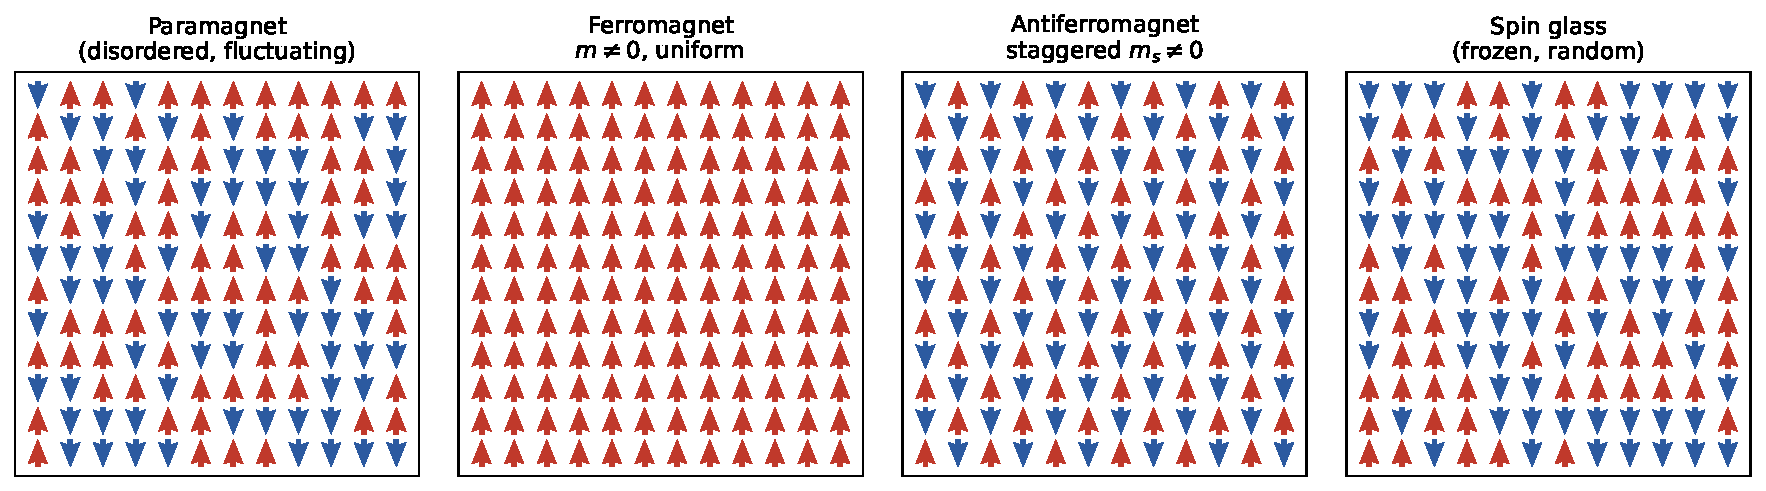
\includegraphics[width=\textwidth]{figs/phases.pdf}
\caption{The four collinear phases as Ising spin configurations (red $=$ up,
blue $=$ down). The paramagnet and the spin glass look alike in a single snapshot --
their difference is \emph{dynamical}: paramagnet spins fluctuate freely, spin-glass
spins are frozen into one random pattern. This is precisely the kind of distinction a
learned representation can capture and a naive eye cannot.}
\label{fig:phases}
\end{figure}

\paragraph{Paramagnet (disordered).} At high $T$ thermal fluctuations win; spins point
every which way and average to zero, $m=0$. No symmetry is broken. Susceptibility
follows the Curie--Weiss law $\chi\propto 1/(T-\theta_{\mathrm{CW}})$.

\paragraph{Ferromagnet.} Below the Curie temperature $T_c$ the spins align, giving
$m\neq0$ and macroscopic magnetization. The $\mathbb{Z}_2$ (up/down) or $O(n)$ rotational
symmetry of Eq.~\eqref{eq:exchange} is spontaneously broken. Examples: Fe, Co, Ni.

\paragraph{Antiferromagnet and ferrimagnet.} With $J<0$, neighbours anti-align into a
staggered (N\'eel) pattern; the net moment is zero but $m_s\neq0$ below the N\'eel
temperature $T_N$. If the two sublattices have unequal moments the leftover is a
\emph{ferrimagnet} (e.g.\ magnetite). Examples: MnO, NiO.

\paragraph{Frustration and noncollinear order.} When the lattice geometry forbids
satisfying every bond simultaneously the system is \emph{frustrated}
(Fig.~\ref{fig:frust}a). The classic case is three antiferromagnetically coupled spins
on a triangle: no arrangement makes all three pairs antiparallel. The compromise is
often a noncollinear state such as the $120^\circ$ order of the triangular-lattice
antiferromagnet (Fig.~\ref{fig:frust}b). Frustration is the gateway to spin glasses,
spin liquids and skyrmions.

\begin{figure}[h]
\centering
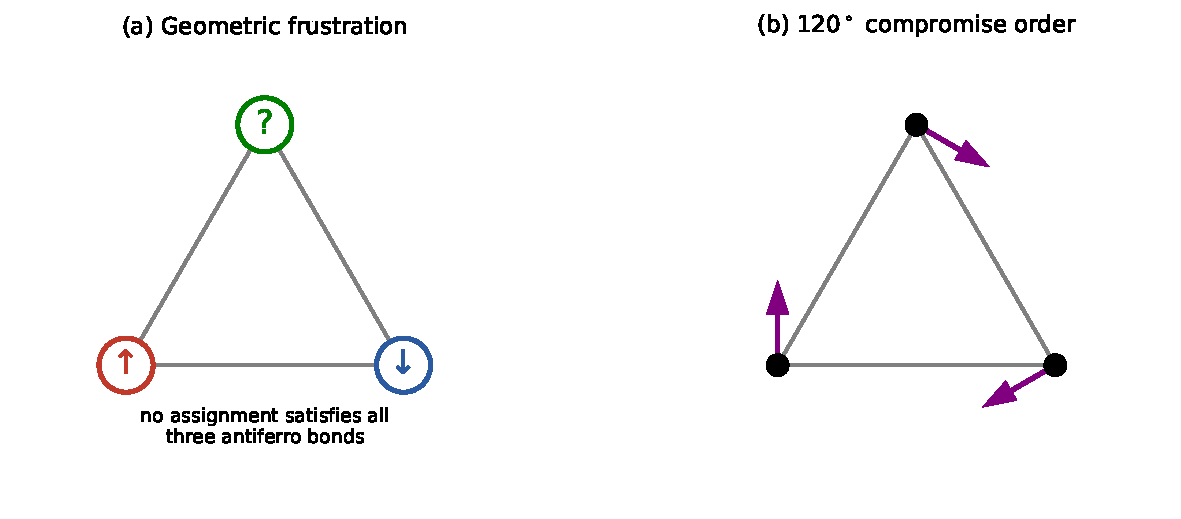
\includegraphics[width=0.82\textwidth]{figs/frustration.pdf}
\caption{Geometric frustration. (a) On a triangle with antiferromagnetic bonds the
third spin cannot satisfy both of its neighbours. (b) The system resolves the conflict
with a noncollinear $120^\circ$ compromise -- an ordered but non-trivial ground state.}
\label{fig:frust}
\end{figure}

\paragraph{Spin glass.} With \emph{quenched randomness} in the couplings (random $J_{ij}$
of both signs, as in the Edwards--Anderson model) the spins freeze into a random,
frustrated pattern with no periodic order. The order parameter is not a magnetization
but the Edwards--Anderson overlap $q_{\mathrm{EA}}=\frac1N\sum_i\langle S_i\rangle^2$,
measuring how frozen each spin is. Spin glasses have a rugged free-energy landscape with
many nearly degenerate minima -- the reason they are computationally brutal (and, not
coincidentally, why spin-glass theory underlies both optimization and neural networks).

\paragraph{Skyrmions: topological textures.} The Dzyaloshinskii--Moriya interaction
twists neighbouring spins, stabilising nanoscale swirls called \emph{magnetic skyrmions}
(Fig.~\ref{fig:sky}). A skyrmion is \emph{topologically protected}: its spins wrap the
unit sphere an integer number of times,
\begin{equation}
Q=\frac{1}{4\pi}\!\int\! \mathbf{m}\cdot(\partial_x\mathbf{m}\times\partial_y\mathbf{m})\,dx\,dy \;\in\;\mathbb{Z},
\end{equation}
and cannot be smoothly unwound. In chiral magnets (MnSi, FeGe) skyrmions crystallise into
a lattice inside a small pocket of the field--temperature phase diagram
(Fig.~\ref{fig:pd}). Because they are small, stable and current-drivable, they are a
leading candidate for racetrack memory -- the applied, device-physics end of magnetism.

\begin{figure}[h]
\centering
\begin{minipage}[c]{0.46\textwidth}\centering
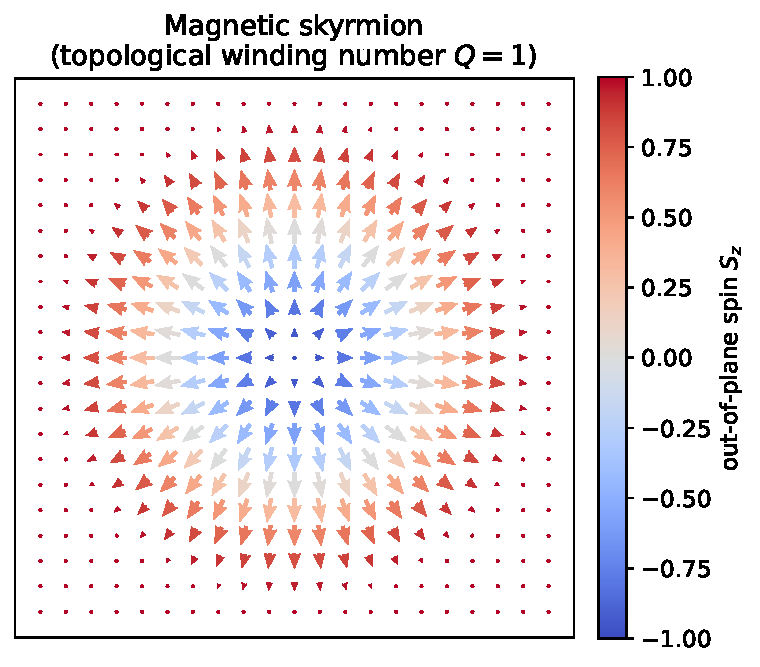
\includegraphics[width=\textwidth]{figs/skyrmion.pdf}
\end{minipage}\hfill
\begin{minipage}[c]{0.5\textwidth}\centering
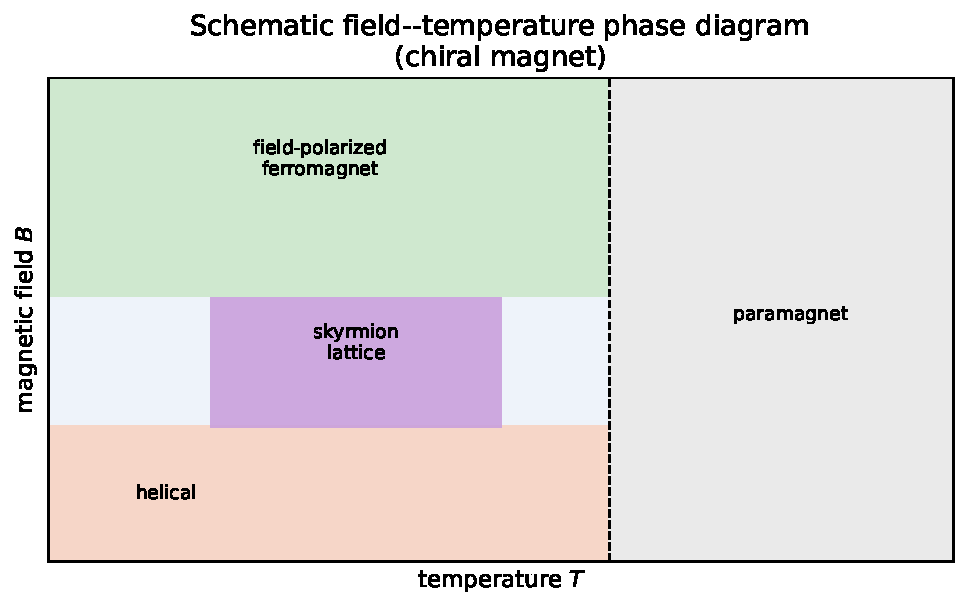
\includegraphics[width=\textwidth]{figs/phasediagram.pdf}
\end{minipage}
\caption{\emph{Left:} a N\'eel skyrmion -- in-plane spins (arrows) rotate from
down at the core to up at the rim; colour is the out-of-plane component $S_z$.
\emph{Right:} skyrmions occupy a small pocket of the $B$--$T$ phase diagram of a chiral
magnet, bordered by helical/spiral, field-polarised, and paramagnetic phases.}
\label{fig:sky}
\end{figure}
\addtocounter{figure}{-1}\refstepcounter{figure}\label{fig:pd}

\paragraph{Quantum spin liquid.} In strongly frustrated \emph{quantum} magnets, quantum
fluctuations can prevent order down to $T=0$: the spins remain collectively entangled and
fluctuating -- a \emph{spin liquid}. There is no local order parameter; the phase is
diagnosed by long-range entanglement, fractionalised excitations, and topological order.
Candidate materials include the kagome antiferromagnet herbertsmithite and Kitaev
material $\alpha$-RuCl$_3$. This is the hardest phase to identify, classically or with ML,
and a major frontier.

% ======================================================================
\section{Phase transitions and criticality}
% ======================================================================
Approaching $T_c$ from below, the order parameter vanishes continuously and response
functions diverge (Fig.~\ref{fig:op}). Near a continuous transition, observables obey
\emph{power laws} governed by \emph{critical exponents},
\begin{equation}
m\sim (T_c-T)^{\beta},\qquad
\chi\sim |T-T_c|^{-\gamma},\qquad
\xi\sim |T-T_c|^{-\nu},
\end{equation}
where $\xi$ is the correlation length. The susceptibility is fixed by fluctuations,
$\chi=\beta\big(\langle M^2\rangle-\langle M\rangle^2\big)/N$. Remarkably, the exponents
depend only on symmetry and dimension, not microscopic detail --
\emph{universality}. The 2D Ising model is exactly solvable (Onsager 1944) with
$\beta=1/8,\ \gamma=7/4,\ \nu=1$, which is why it is the perfect ML benchmark: the ground
truth is known in closed form.

\begin{figure}[h]
\centering
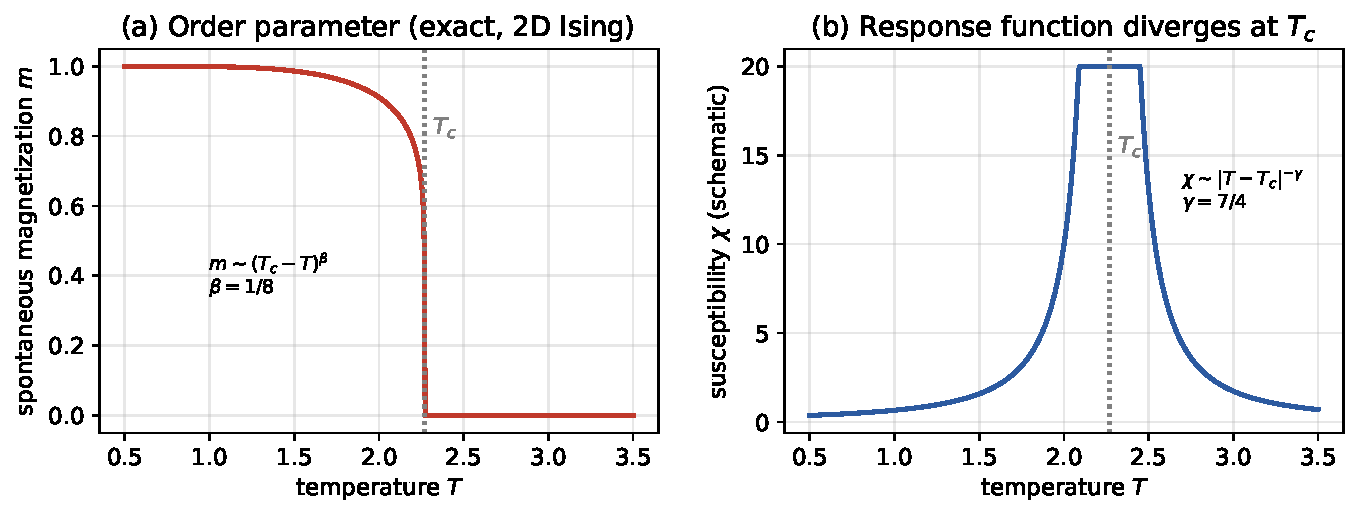
\includegraphics[width=0.9\textwidth]{figs/orderparam.pdf}
\caption{(a) Exact 2D-Ising spontaneous magnetization $m(T)=\big[1-\sinh^{-4}(2\beta
J)\big]^{1/8}$ vanishing at $T_c$ with exponent $\beta=1/8$. (b) The susceptibility
diverges at $T_c$ (schematic $\gamma=7/4$).}
\label{fig:op}
\end{figure}

\paragraph{A transition without a local order parameter: BKT.} The 2D XY model has a
continuous symmetry and \emph{no} conventional ordered phase, yet it undergoes the
Berezinskii--Kosterlitz--Thouless transition driven by the binding and unbinding of
\emph{vortices} (Fig.~\ref{fig:vortex}). Below $T_{\mathrm{BKT}}$ vortices bind into
neutral pairs; above it they proliferate and destroy quasi-order. BKT is the paradigm of
a \emph{topological} phase transition -- and precisely the kind of subtle transition
where an unsupervised network, having no built-in notion of ``magnetization'', can still
detect the change.

\begin{figure}[h]
\centering
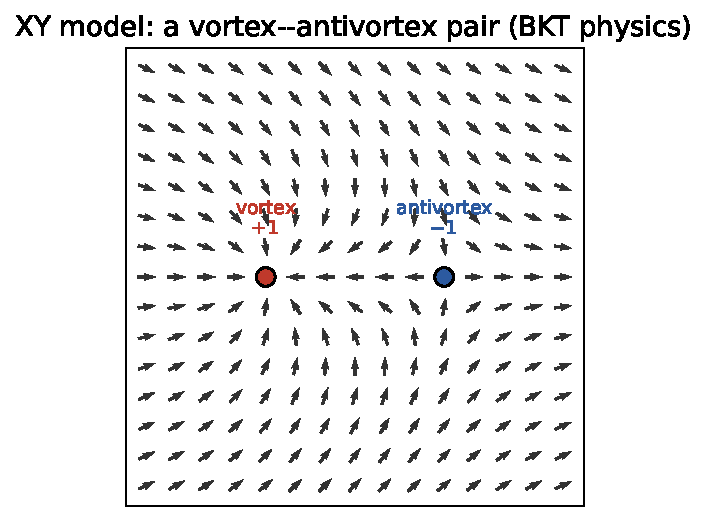
\includegraphics[width=0.62\textwidth]{figs/vortex.pdf}
\caption{A vortex ($+1$) and antivortex ($-1$) in the XY model. The BKT transition is the
unbinding of such pairs; there is no local order parameter, so it defies naive
order-parameter thinking and motivates learned detectors.}
\label{fig:vortex}
\end{figure}

\paragraph{Critical slowing down -- the crux for computation.} Near $T_c$ the correlation
length $\xi$ diverges, and any \emph{local} Monte Carlo update (flip one spin, accept/reject)
takes a diverging number of steps to produce an independent configuration:
\begin{equation}
\tau_{\mathrm{int}}\sim \xi^{\,z}\sim |T-T_c|^{-\nu z},
\end{equation}
with dynamic exponent $z\approx2$ for single-spin dynamics. Independent samples become
extraordinarily expensive exactly where the interesting physics lives. This single fact
is the doorway through which one class of ML methods enters (Sec.~\ref{sec:van}).

% ======================================================================
\section{Why classical tools struggle (and where ML helps)}
% ======================================================================
Before ML, three workhorses dominate, each with a hard wall:
\begin{itemize}
\item \textbf{Monte Carlo} samples $p(s)\propto e^{-\beta E(s)}$ with a Markov chain.
Wall: \emph{critical slowing down} near $T_c$ (partly cured by cluster algorithms such as
Wolff/Swendsen--Wang, but not for generic frustrated or continuous-spin models).
\item \textbf{Exact diagonalization} of quantum models is exact but limited to
$\sim\!40$ spins by the $2^N$ Hilbert space.
\item \textbf{Quantum Monte Carlo} handles large quantum systems -- until the
\emph{sign problem} makes frustrated or fermionic models exponentially hard.
\end{itemize}
Machine learning does not repeal these walls, but it offers new \emph{representations} and
\emph{samplers} that sometimes scale better or need no hand-crafted order parameter. The
rest of the document maps those methods.

% ======================================================================
\section{How AI attaches to magnetism: a taxonomy}
% ======================================================================
There are five distinct ways ML enters, and they answer genuinely different questions.
Table~\ref{tab:map} is the summary; the subsections give the mechanics.

\begin{table}[h]
\centering\small
\caption{Five ways machine learning attaches to magnetic models.}
\label{tab:map}
\begin{tabular}{@{}p{3.5cm}p{4.3cm}p{4.6cm}p{2.4cm}@{}}
\toprule
Method & Question it answers & How & Phase target \\
\midrule
Supervised classifier (CNN/GNN) & ``Which phase is this configuration?'' & Train on labelled snapshots; net learns the decision boundary & FM/AFM/PM \\[2pt]
Unsupervised (PCA, VAE) & ``Is there a transition, and what is the order parameter?'' & Learn latent structure without labels; clusters $=$ phases & any, incl.\ hidden \\[2pt]
Generative sampler (VAN) & ``Give me independent samples and the free energy.'' & Autoregressive net trained to variational free energy & classical, near $T_c$ \\[2pt]
Neural quantum state & ``What is the ground state of this quantum magnet?'' & Wavefunction $=$ neural net, minimise energy & spin liquids \\[2pt]
PINN / neural operator & ``Solve the magnetisation dynamics / screen materials.'' & Encode LLG PDE as a loss; or map structure$\to$property & skyrmions, discovery \\
\bottomrule
\end{tabular}
\end{table}

% ---------------------------------------------------------------
\subsection{Supervised phase classification}
The most direct idea (Carrasquilla \& Melko 2017): treat a spin configuration as an image,
label it by its known phase, and train a convolutional network to predict the label. The
network discovers the relevant features on its own, and the point where its output
probability crosses $1/2$ pinpoints $T_c$.

\begin{center}
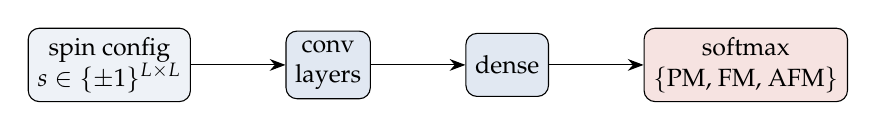
\begin{tikzpicture}[node distance=9mm and 12mm,
  box/.style={draw,rounded corners,minimum height=8mm,align=center,font=\small},
  every path/.style={-{Stealth[length=2mm]}}]
\node[box,fill=acc!8] (in) {spin config\\ $s\in\{\pm1\}^{L\times L}$};
\node[box,right=of in,fill=acc!14] (c1) {conv\\ layers};
\node[box,right=of c1,fill=acc!14] (d1) {dense};
\node[box,right=of d1,fill=acc2!14] (out) {softmax\\ $\{$PM, FM, AFM$\}$};
\draw (in)--(c1); \draw (c1)--(d1); \draw (d1)--(out);
\end{tikzpicture}
\end{center}
\noindent \emph{Strength:} simple, accurate. \emph{Weakness:} needs labels, i.e.\ you must
already know the phases -- so it confirms rather than discovers.

% ---------------------------------------------------------------
\subsection{Unsupervised discovery of order parameters}
Here we hand the network \emph{unlabelled} configurations and ask it to find structure.
The simplest such method, principal component analysis, already works for the Ising model:
the leading principal component of raw spin snapshots \emph{is} the magnetization
(Wang 2016). Figure~\ref{fig:pca} shows this computed from scratch -- PCA was never told
about temperature or magnetization, yet PC1 recovers the order parameter and separates the
phases.

\begin{figure}[h]
\centering
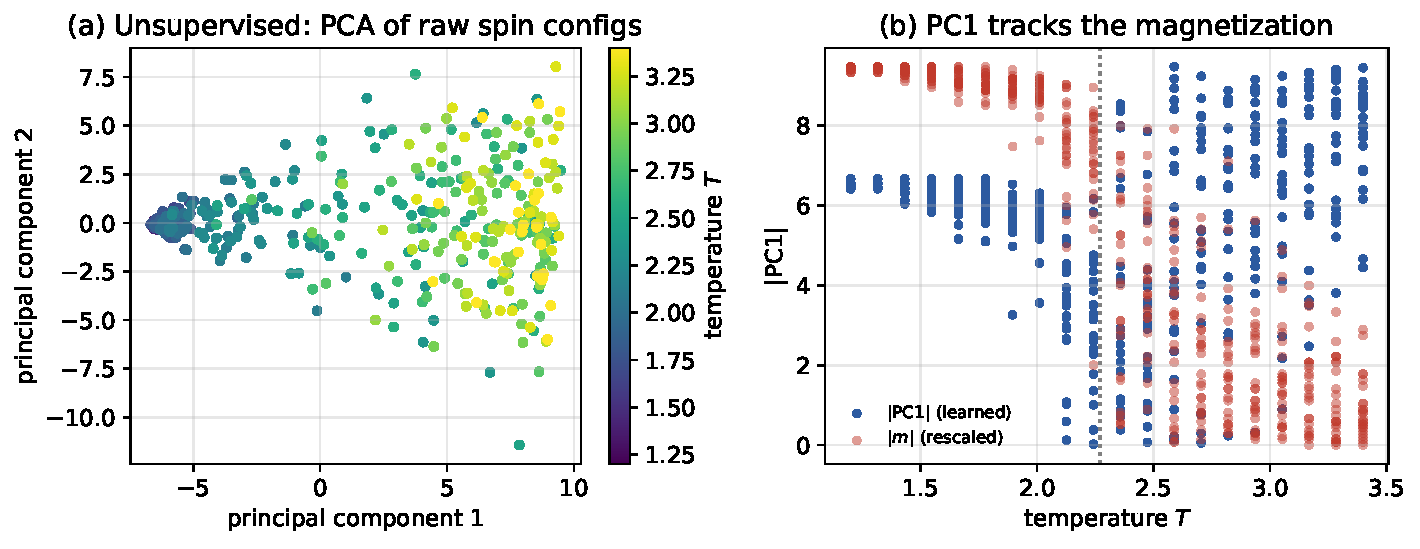
\includegraphics[width=0.92\textwidth]{figs/pca.pdf}
\caption{Unsupervised learning, computed here on Monte Carlo Ising configurations
($L=16$). (a) Projecting raw spin snapshots onto their first two principal components;
colour is temperature, which the algorithm never saw. Ordered (cold) configurations
spread along PC1; disordered (hot) ones collapse near the origin. (b) $|$PC1$|$ tracks the
true magnetization and drops near $T_c$ -- a \emph{machine-discovered} order parameter.}
\label{fig:pca}
\end{figure}

\noindent Nonlinear versions -- autoencoders and \emph{variational autoencoders} (VAEs) --
extend this to phases where PCA fails, learning a low-dimensional latent code whose
clustering reveals the phase diagram. This is the ideal ``discovery'' tool for exotic order
(chiral, topological) where no human order parameter is known: the physicist supplies the
Hamiltonian and the ground truth; the network proposes the coordinate.

% ---------------------------------------------------------------
\subsection{Generative sampling: Variational Autoregressive Networks}
\label{sec:van}
This is the method that directly attacks critical slowing down, and the core of our joint
project. Instead of a Markov chain we build a normalised neural distribution $q_\theta(s)$
written \emph{autoregressively}, so that each spin's probability is conditioned on the
previous ones:
\begin{equation}
q_\theta(s)=\prod_{k=1}^{N} q_\theta\!\left(s_k \mid s_1,\dots,s_{k-1}\right).
\end{equation}

\begin{center}
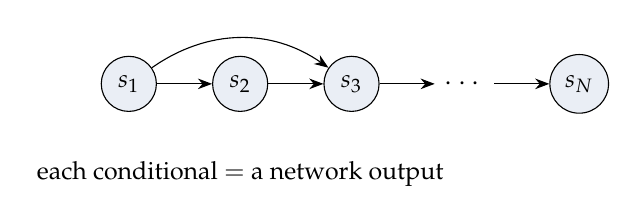
\begin{tikzpicture}[node distance=7mm,
  s/.style={draw,circle,minimum size=7mm,font=\small,fill=acc!10},
  every path/.style={-{Stealth[length=1.8mm]}}]
\node[s](s1){$s_1$};\node[s,right=of s1](s2){$s_2$};
\node[s,right=of s2](s3){$s_3$};\node[right=of s3](d){$\cdots$};
\node[s,right=of d](sn){$s_N$};
\draw (s1)--(s2);\draw[bend left=35] (s1) to (s3);\draw (s2)--(s3);
\draw (s3)--(d);\draw (d)--(sn);
\node[below=5mm of s2,font=\small,align=center] {each conditional $=$ a network output};
\end{tikzpicture}
\end{center}

\noindent Two properties fall out for free: we can \textbf{sample exactly} (one sequential
pass, i.i.d.\ configurations) and \textbf{evaluate $q_\theta(s)$ exactly}. We train by
minimising the \emph{variational free energy}
\begin{equation}
\beta F_q=\mathbb{E}_{s\sim q}\!\big[\beta E(s)+\ln q_\theta(s)\big]
=\beta F_{\text{exact}}+D_{\mathrm{KL}}(q\,\|\,p)\;\ge\;\beta F_{\text{exact}},
\end{equation}
which is a \emph{rigorous upper bound} -- the network hands you a certified free energy,
something ordinary MC does not. Because spins are discrete we use the score-function
(REINFORCE) gradient with a baseline $b$,
\begin{equation}
\nabla_\theta(\beta F_q)=\mathbb{E}_{s\sim q}\!\big[(\beta E(s)+\ln q_\theta(s)-b)\,\nabla_\theta\ln q_\theta(s)\big].
\end{equation}
Since every sample is independent, the autocorrelation time is $\tau_{\mathrm{int}}=1$ at
\emph{all} temperatures -- critical slowing down is gone by construction
(Fig.~\ref{fig:csd}). Figure~\ref{fig:van} shows our own $L=8$ run reproducing the exact
Onsager thermodynamics.

\begin{figure}[h]
\centering
\begin{minipage}[c]{0.52\textwidth}\centering
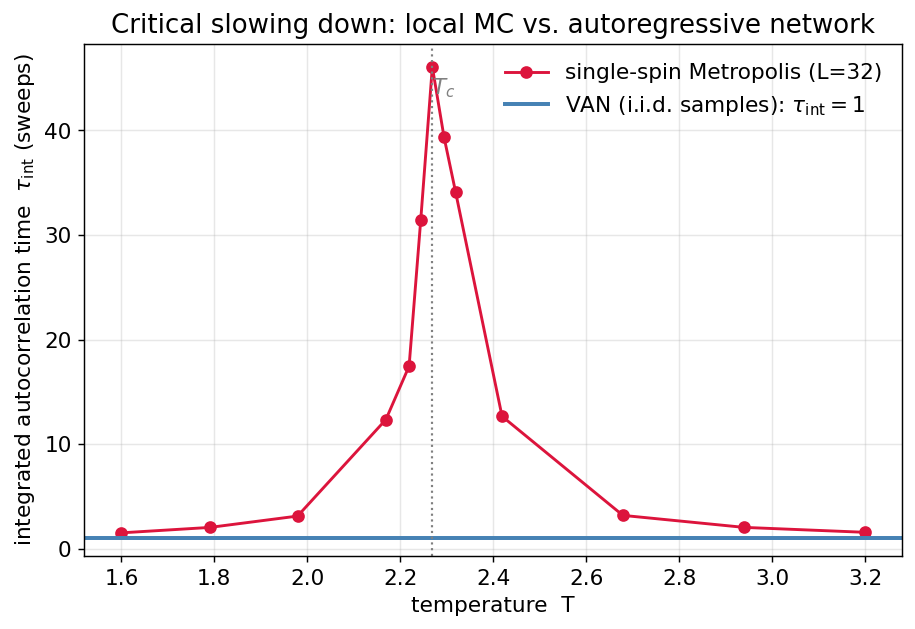
\includegraphics[width=\textwidth]{figs/csd.png}
\end{minipage}\hfill
\begin{minipage}[c]{0.44\textwidth}\centering
\caption{Critical slowing down made visible (our computation). Single-spin Metropolis
autocorrelation time $\tau_{\mathrm{int}}$ spikes at $T_c$ (here to $\sim\!46$ sweeps,
$L=32$); a variational autoregressive network draws independent samples, so
$\tau_{\mathrm{int}}=1$ everywhere.}
\label{fig:csd}
\end{minipage}
\end{figure}

\begin{figure}[h]
\centering
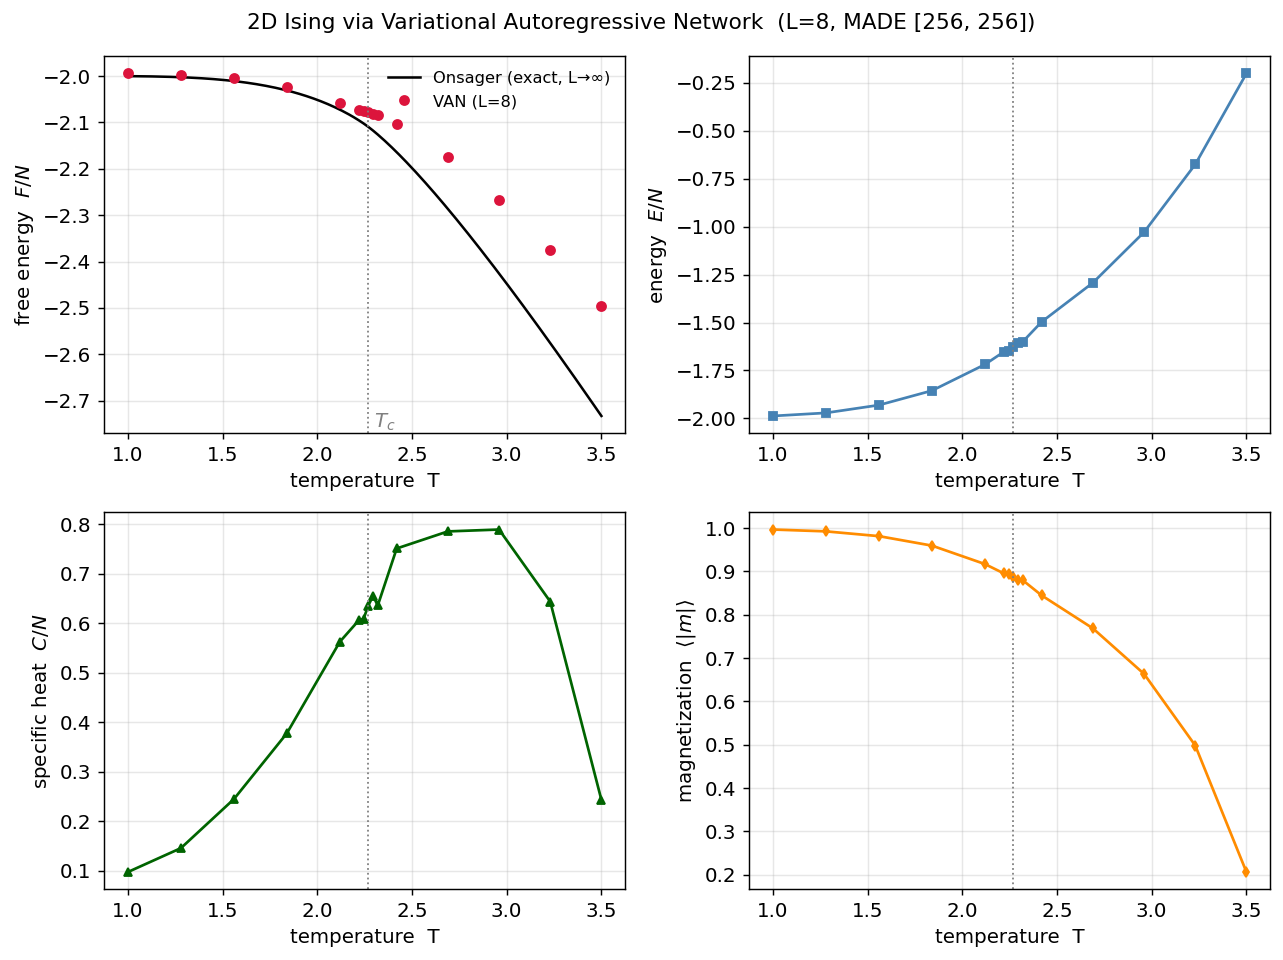
\includegraphics[width=0.95\textwidth]{figs/vanthermo.png}
\caption{Our from-scratch VAN ($L=8$) versus the exact Onsager solution: the free energy
respects the variational bound (points sit above the exact curve) and the energy, specific
heat and magnetization reproduce the ordering crossover near $T_c$.}
\label{fig:van}
\end{figure}

\paragraph{The bridge to radiation transport.} VAN training is \emph{importance sampling
with a learned proposal}: $q_\theta$ is the biased sampling distribution and $\ln q$ is the
log-weight -- the same weight bookkeeping as weight-window variance reduction in
Monte Carlo particle transport, but in configuration space instead of phase space. The
variational free-energy bound is the analogue of an unbiased weighted estimator. This is a
genuine conceptual overlap with deep-penetration shielding work, not a superficial one.

% ---------------------------------------------------------------
\subsection{Neural quantum states: ground states of quantum magnets}
For \emph{quantum} magnets the object of interest is the ground-state wavefunction
$\psi(s)=\langle s|\psi\rangle$ over the $2^N$ basis states. Carleo \& Troyer (2017)
proposed representing $\psi_\theta(s)$ by a neural network and minimising the variational
energy
\begin{equation}
E[\theta]=\frac{\langle\psi_\theta|H|\psi_\theta\rangle}{\langle\psi_\theta|\psi_\theta\rangle}\;\ge\;E_0 ,
\end{equation}
by stochastic sampling of $|\psi_\theta(s)|^2$.

\begin{center}
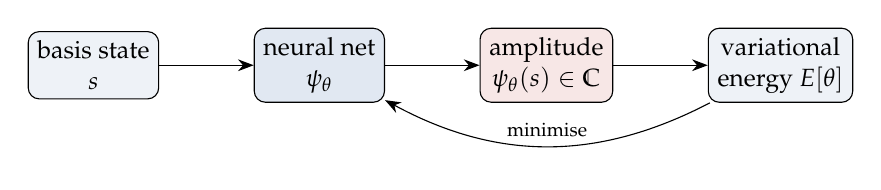
\begin{tikzpicture}[node distance=8mm and 12mm,
  box/.style={draw,rounded corners,minimum height=8mm,align=center,font=\small},
  every path/.style={-{Stealth[length=2mm]}}]
\node[box,fill=acc!8](in){basis state\\ $s$};
\node[box,right=of in,fill=acc!14](nn){neural net\\ $\psi_\theta$};
\node[box,right=of nn,fill=acc2!12](amp){amplitude\\ $\psi_\theta(s)\in\mathbb{C}$};
\node[box,right=of amp,fill=acc!8](e){variational\\ energy $E[\theta]$};
\draw(in)--(nn);\draw(nn)--(amp);\draw(amp)--(e);
\draw[bend left=28] (e) to node[above,font=\scriptsize]{minimise} (nn);
\end{tikzpicture}
\end{center}
\noindent The frontier target is the frustrated / spin-liquid regime where the wavefunction
has a hard \emph{sign structure} (the ``sign problem'' resurfacing). The ML challenges are
architectures that enforce lattice and spin symmetries and represent signs -- restricted
Boltzmann machines, autoregressive/RNN wavefunctions, and transformers. This is the
highest-ceiling, most competitive direction; enter it only with a physics insight others
lack.

% ---------------------------------------------------------------
\subsection{PINNs, neural operators, and materials discovery}
Two applied directions round out the map. \textbf{Physics-informed neural networks} (Raissi
et al.\ 2019) solve the Landau--Lifshitz--Gilbert equation of micromagnetics,
\begin{equation}
\frac{d\mathbf{m}}{dt}=-\gamma\,\mathbf{m}\times\mathbf{H}_{\mathrm{eff}}
+\alpha\,\mathbf{m}\times\frac{d\mathbf{m}}{dt},
\end{equation}
by encoding the PDE residual as a training loss -- useful for skyrmion nucleation and
domain dynamics; \emph{neural operators} instead learn the whole map from material
parameters to the equilibrium texture, replacing expensive solvers. \textbf{Graph neural
networks} (Xie \& Grossman 2018) take a crystal structure as a graph and predict magnetic
ground state and ordering temperature, enabling high-throughput screening for
rare-earth-free room-temperature ferromagnets; large-scale efforts of this kind (e.g.\
GNoME, 2023) have expanded known stable materials by orders of magnitude.

% ======================================================================
\section{Putting it together: our roadmap}
% ======================================================================
The methods above are not equally ripe for a two-person team. Ordered by realism:
\begin{enumerate}
\item \textbf{Paper 1 -- VAN for the classical Ising model, scaled up} ($L=16,32,64$).
Headline: elimination of critical slowing down plus a certified free-energy bound.
Working code and the figures in this document already exist.
\item \textbf{Paper 2 -- the XY model and the BKT transition.} Same machinery, a
continuous-spin energy, a topological transition with no local order parameter -- higher
physics interest, modest new ML.
\item \textbf{Stretch -- neural quantum states for a frustrated magnet.} High ceiling,
crowded field; pursue only where a specific physics insight gives an edge.
\end{enumerate}

\paragraph{Division of labour.} \emph{Physics (you):} define Hamiltonians and phase
diagrams, guarantee ground truth (Onsager, enumeration, exact diagonalization), interpret
what the network learns, and own the importance-sampling / variance-reduction narrative.
\emph{ML (collaborator):} architectures (MADE $\to$ PixelCNN $\to$ transformer;
symmetry-equivariant layers), optimisation (REINFORCE variance reduction, natural gradient,
schedules), and scaling/engineering.

% ======================================================================
\section*{Appendix: one-line glossary}
\addcontentsline{toc}{section}{Appendix: one-line glossary}
\small
\begin{itemize}
\item \textbf{Order parameter} -- zero in the disordered phase, nonzero once a symmetry breaks.
\item \textbf{Universality} -- critical exponents depend only on symmetry and dimension.
\item \textbf{Frustration} -- geometry/couplings forbid satisfying all bonds at once.
\item \textbf{Critical slowing down} -- local MC decorrelation time diverges at $T_c$ ($\tau\sim\xi^z$).
\item \textbf{Sign problem} -- oscillating signs make frustrated/fermionic QMC exponentially hard.
\item \textbf{Variational free energy} -- $\beta F_q=\mathbb{E}_q[\beta E+\ln q]\ge\beta F_{\text{exact}}$; the VAN loss.
\item \textbf{Topological order / winding} -- integer-valued, robust to smooth deformation (skyrmion $Q$, vortex charge).
\end{itemize}

% ======================================================================
\section*{Key references}
\addcontentsline{toc}{section}{Key references}
\small
\begin{enumerate}[itemsep=1pt]
\item L.\ Onsager, \emph{Crystal statistics I}, Phys.\ Rev.\ \textbf{65}, 117 (1944) -- exact 2D Ising.
\item J.\ Kosterlitz \& D.\ Thouless, J.\ Phys.\ C \textbf{6}, 1181 (1973) -- BKT transition.
\item S.\ Edwards \& P.\ Anderson, J.\ Phys.\ F \textbf{5}, 965 (1975) -- spin-glass model.
\item S.\ M\"uhlbauer et al., Science \textbf{323}, 915 (2009) -- skyrmion lattice in MnSi.
\item J.\ Carrasquilla \& R.\ Melko, Nat.\ Phys.\ \textbf{13}, 431 (2017) -- ML phases of matter.
\item L.\ Wang, Phys.\ Rev.\ B \textbf{94}, 195105 (2016) -- unsupervised discovery of transitions.
\item G.\ Carleo \& M.\ Troyer, Science \textbf{355}, 602 (2017) -- neural quantum states.
\item D.\ Wu, L.\ Wang \& P.\ Zhang, Phys.\ Rev.\ Lett.\ \textbf{122}, 080602 (2019) -- variational autoregressive networks.
\item M.\ Raissi, P.\ Perdikaris \& G.\ Karniadakis, J.\ Comput.\ Phys.\ \textbf{378}, 686 (2019) -- physics-informed neural networks.
\item T.\ Xie \& J.\ Grossman, Phys.\ Rev.\ Lett.\ \textbf{120}, 145301 (2018) -- crystal graph networks for materials.
\end{enumerate}

\end{document}
